%!TEX root = ../3dbook.tex

\setchapterpreamble[u]{\margintoc}

\graphicspath{{bim/}}
% \renewcommand*{\thelesson}{7.2}

\chapter{Building information models}%
\label{chap:bim}

Building information model (BIM) involves the creation and use of detailed digital 3D models of buildings or infrastructure in a way that supports their design and construction, but increasingly also extending to their planning, operation, maintenance, refurbishing and/or demolition.

Originally, the scope of BIM was limited to support a building's design and construction in the Architecture Engineering and Construction (AEC) field.
However, BIM models are now considered to be useful for much more than this narrow purpose, representing a central platform that can be used throughout a building's entire lifecycle, supporting collaboration by different users and different disciplines.
For example, the most typical current use of BIM comprises the design phase of a building, where different domain experts (\eg\ architectural design, structural design and installations design) can work together to create one comprehensive 3D model that contains all elements of a building.
Later on, the same model could be maintained to support the building's asset and facility management.

In industry, the potential of BIM is commonly focussed on improving existing processes (\eg\ minimising errors during design and construction, optimising resources, improving coordination and control).
However, there is a lot of ongoing work to reuse BIM models for new applications (\eg\ structural analysis, energy simulations, urban planning and building permitting).
These applications often imply the conversion and integration of BIM models with other sources, such as 3D city models.
%By contrast, a common academic/government view is that BIM is mainly about the 3D models themselves, and thus it is important that they reflect the real situation as much as possible.
% In this latter view, the improved processes and new applications are simply the result of using these models in a smart way.
% This is why it is relevant to know and manage such a different kind of 3D model.



\section{How BIM came to be}

Traditionally, the design of buildings and infrastructure mostly relied on technical drawings on paper, often as a combination of more engineering-focused 2D cross-sections and floor plans, with more visual drawings (\eg\ architectural sketches) that showed an overview of project as 2D perspective views, either in a stylised or in a realistic way.
These were sometimes supplemented with 3D physical models (\ie\ maquettes).

Although the initial concept of BIM was developed starting from the 1980s, when these design processes were (partly) transferred to computers, it mostly meant the use of 2D computer-aided design (CAD) software to create the technical drawings and the use of general-purpose graphics editing software for the other views.
While this simplified many tasks (\eg\ iterating to make small changes and printing new versions), it is worth noting that the use of these kinds of software did not fundamentally change the nature of designing a building, or of using the archived versions of such designs for later purposes (\eg\ locating pipes and wires), which were most likely only stored in print anyway.

BIM is often considered as an evolution from these CAD-based processes, which is partly true, but it is also a very different way to model buildings and infrastructure.
This is mainly because it models a building or infrastructure project as a single model composed of a large set of 3D objects, as opposed to a series of unconnected 2D drawings showing different views of subsets of these objects.
The kind of technical drawings that were made before are still common, but they can be semi-automatically generated from the BIM model using software.

The objects represented in a BIM model include the 3D elements that a building is composed of (\eg\ beams, columns, stairs and windows).
They can range from higher level representations (less detailed) up to the representation of detailed single screws, with their accompanying relevant attributes (\eg\ the materials they are made of and their properties).
Moreover, more abstract elements are included that describe the project itself (\eg\ construction timelines and costs).
There is also a large number of relations between the objects, which are often used by software to support smart editing features, such as keeping sets of related objects together when one of them is moved.

Note that a key aspect of BIM is that it focusses on volume-filling physical objects (Figure~\ref{fig:volumetric}), such as walls, whereas GIS representations instead tend to model the objects' outer surfaces (\eg\ wall surfaces) and the voids between them (\eg\ rooms).
This means that BIM models are usually more detailed and have semantics that are more meaningful for some purposes (\eg\ construction or refurbishing), but 3D GIS models have higher-level semantics that are easier for many applications (\eg\  navigation and spatial analyses).
Table~\ref{tab:vs} compares the ways in which in 3D city models and BIM models differ.

\begin{figure}
\centering
\includegraphics[width=\linewidth]{figs/volumetric.pdf}
\caption{BIM models focus on volumetric physical elements (centre), whereas 3D GIS models focus on semantic surfaces (left) and the voids between them (right).}%
\label{fig:volumetric}
\end{figure}

\begin{table}
	\centering
	\small
	\begin{tabular}{m{2.3cm}m{3.5cm}m{3.5cm}}
		\toprule
		& \textbf{3D city models} & \textbf{BIM}  \\ \midrule
		geometry & boundary representation (explicit) & parametrically modelled solids (implicit) \\ \addlinespace 
		data source & surveys & designs \\ \addlinespace 
		range of detail ($d$) & $1000>d>0.1$ m & $50>d>0.001$ m \\ \addlinespace 
		semantics & city/terrain & building elements  \\ \addlinespace 
		georeferencing & compulsory & optional  \\ \addlinespace 
		analysis & city-level & building-level \\ \addlinespace 
		evolution of & GIS & CAD \\ \addlinespace 
		dominated by & government & industry \\ \bottomrule
	\end{tabular}
	\caption{Comparison between 3D city models features and BIM aspects.}%
	\label{tab:vs}
\end{table}

\subsection{Use of BIM and common terminology}

BIM was originally focussed on the design of buildings, but its reach has expanded significantly in recent years and is continuing to do so in a number of ways.
Firstly, it is attempting to cover all sorts of non-building infrastructure projects as well, including roads, railways, bridges, tunnels, waterways, utility and communication networks, which together with buildings are often known as \emph{assets}.
Secondly, it also aims to support all the stages of the lifecycle of an asset using the same base data, including its planning (with the help of GIS data), design, construction, operation, maintenance, refurbishing and demolition.
These stages will likely involve different software, \eg\ specialised building design and asset management software; and it will also likely involve different people, \eg\ architects, surveyors, civil engineers, etc.

Relevant to this, some software vendors and organisations (\eg\ the American Institute of Architects and the UK BIM Task Group) have come up with the concept of the level of development (LOD) of a BIM model, which is equivalent to the concept of level of detail (also LOD or LoD) in GIS\@.
While both terms are directly related to how abstract a model is, and indirectly to how complex the geometries in it are, the two terms are somewhat different.
Different LoDs in GIS usually model the same features at the same time, but they are captured at or generalised to different levels of detail.
Different LODs in a BIM model instead show the same asset at the different stages that it goes through, from its conception (as a rough sketch or even with no geometry), and gaining more detail as it passes through its design and to its construction.
Ideally, this extends to modification of the model to reflect its as-built state, which can be then used for asset management and other applications.
The exact terms used for different BIM LODs differ, but a common scheme is from LOD 100 (concept), LOD 200 (design during development), LOD 300 (detailed design to calculate materials and costs), LOD 400 (construction) and LOD 500 (asset management).
Other schemes use smaller numbers, such as 1 to 7 in the United Kingdom, or use the same hundreds-series numbers but with different definitions.

In the recent ISO 19560 standard (Organization and digitization of information about buildings and civil engineering works, including building information modelling (BIM) --- Information management using building information modelling), the Level of Information Need (LOIN) is defined as a `framework which defines the extent and granularity of information' and is intended to substitute the many and inconsistent previous classifications of LODs in BIM\@.
The LOIN is intended for clients who define their information needs for project management: various metrics can be used to measure the information to be delivered.
For example, geometry, alphanumeric data and documents, as well as unstructured information such as plans, reports, photographs and so on, with the alphanumeric information considered at least as important as geometry, helping in the process of passing from documents (reports, manuals, product specification sheets) to the BIM model itself for the description, storage and management of the information related to the building.

Another important set of terms is related to the dimensions in BIM, which are commonly used but they are used inconsistently\@.
In this, practitioners and software vendors very often refer to 4D BIM, which means that a model includes time information, generally in the context of construction scheduling.
Note however that this information might not be in a convenient format, \eg\ a linked Word file with a textual description.
Other dimension definitions sometimes refer to 5D BIM, which usually means a model with cost information.
Finally, different people use 6D or 7D BIM to refer to various other aspects (sustainability, facility management, and delivery of as-built models among others), but the definitions for these are very inconsistent.

Apart from the core applications of BIM in managing a building's lifecycle mentioned above, it is worth noting that there are also many new possibilities that are currently being studied, such as the automatic conversion of BIM models into GIS-ready models that can be integrated into 3D city models, applying environmental analyses directly on BIM models (\eg\ shadow analyses), improving the sustainability of buildings (green BIM), using BIM models to automate building permit issuing, and as will be further discussed in this course, the integration of BIM models with GIS data (GeoBIM).

\section{IFC}

BIM is an industry-dominated field, and software-specific file formats are still the main way in which files are exchanged, such as using the native formats of Autodesk's Revit\marginnote{\url{https://www.autodesk.com/products/revit/overview}} and Graphisoft's ArchiCAD\marginnote{\url{https://www.graphisoft.com/archicad/}} (BIMx).
However, such formats are only well supported by their corresponding software programs, which leads to interoperability problems when exchanging files.

As a way to solve this problem, the buildingSMART consortium, which notably includes a number of software companies (including Autodesk and the Graphisoft-owning Nemetschek Group)\marginnote{\url{https://www.buildingsmart.org/members/member-directory/}}, created the industry foundation classes (IFC)\marginnote{\url{http://www.buildingsmart-tech.org/specifications/ifc-releases}} as an open data model for the exchange of BIM models.
IFC has been further standardised as ISO 16739~\citep{ISO16739:2013} with its geometry definitions in ISO 10303~\citep{ISO10303:2014}.

IFC files are often large (hundreds of MBs), and their structure is rather complex.
They can contain many types of classes (130 defined types, 217 enumeration types, 60 select types, 816 entities, 47 functions, 2 rules, 415 property sets, 93 quantity sets and 1697 individual properties in IFC 4.2\marginnote{\url{https://standards.buildingsmart.org/IFC/DEV/IFC4_2/FINAL/HTML/}}), which are defined using the EXPRESS data modelling language.
Among others, there are several classes to model actors (\eg\ people and organisations), controls (\eg\ specifications, regulations, schedules and other requirements), processes (\eg\ actions during construction), products (\eg\ physical building elements and other spatially defined objects), the project itself (\eg\ where it is placed), and resources (\eg\ cost, materials and equipment), as well as groups of other classes (\eg\ those having a common purpose).
In the rest of this handout, we will mostly focus on products.

\subsection{General organisation of the standard}

The concepts represented in IFC are organized in four conceptual layers, as represented in Figure~\ref{fig:ifclayers}.

\begin{figure}
	\begin{center}
		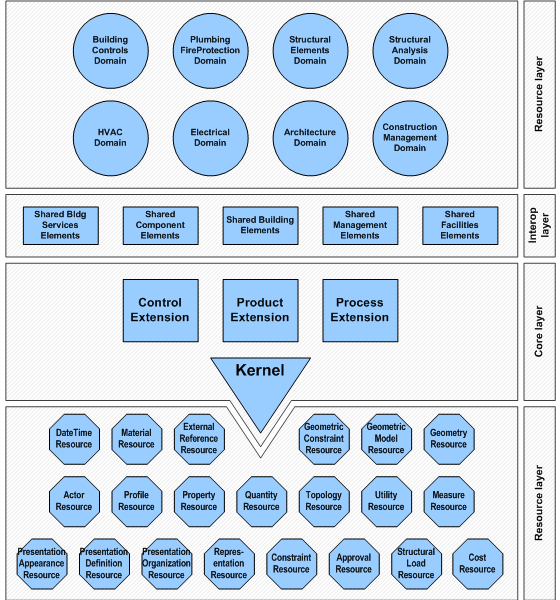
\includegraphics[width=\linewidth]{figs/IFC4LayeredArchitecture.png}
		\caption{{The four layers in which the Industry Foundation Classes are organised. Source: IFC4.1 specification}}%
		\label{fig:ifclayers}
	\end{center}
\end{figure}

The core layer contains the classes which are central and most general in the data model.
In particular, the Kernel contains the root classes for the definition of objects, relationships and properties and their relationships (\eg\ \texttt{IfcRoot}, superclass of all the other entities; \texttt{IfcRelationship}, superclass of all relationships; \texttt{IfcObject}, which is the parent entity of \texttt{IfcGroup}, \texttt{IfcActor}, \texttt{IfcResource}, \texttt{Ifc\-Con\-trol}, \texttt{IfcProcess}, \texttt{IfcProject} and \texttt{IfcProduct}, being specified in the further extensions of the model).
In the core layer there are also the three main extensions representing the foreseen possible representations by IFC:\@ product, control and process.

The interoperability layer includes classes specialising those defined in the \texttt{IfcProductExtension} schema, increasing the level of detail of the represented information. The included entities can be of interest to multiple domains.

Some even more specific information can be represented through the domain specific part of the schema, which can specify either classes represented in the interoperability layer or in the product extension directly (\texttt{IfcArchitectureDomain}, \texttt{IfcBuildingControlsDomain}, \texttt{Ifc\-Cons\-truc\-tion\-Mgmt\-Do\-main}, \texttt{IfcElectricalDomain}, \texttt{IfcHvacDomain}, \texttt{Ifc\-Plum\-bing\-Fire\-Pro\-tec\-tion\-Do\-main}, \texttt{Ifc\-Struc\-tu\-ral\-A\-na\-ly\-sis\-Do\-main}, \texttt{Ifc\-Struc\-tu\-ral\-E\-le\-ments\-Do\-main}).

The resource layer defines entities to further describe the objects defined in the other levels.

\subsection{Formats, encodings and federated models}

The most common encoding of IFC files is the STEP Physical File (SPF), which is a plain text format that is reasonably compact, easy to parse by a computer and human readable (Figure~\ref{fig:step}).
It is also defined in the ISO 10303 standard.
Files with this encoding have the extension \texttt{.ifc}.

\lstset{basicstyle=\footnotesize\ttfamily,breaklines=true}
\begin{figure}
\begin{lstlisting}[frame=single]
#365= IFCDIRECTION((1.,0.,0.));
#367= IFCDIRECTION((0.,0.,1.));
#369= IFCCARTESIANPOINT((0.,0.,0.));
#371= IFCAXIS2PLACEMENT3D(#369,#367,#365);
#372= IFCDIRECTION((0.766044443119,0.642787609687));
#374= IFCGEOMETRICREPRESENTATIONCONTEXT($,'Plan',3,1.00000000000E-5,#371,#372);
#375= IFCGEOMETRICREPRESENTATIONSUBCONTEXT('Box','Plan',*,*,*,*,#374,$,.PLAN_VIEW.,$);
#377= IFCCARTESIANPOINT((-3.,-3.,-1.));
#379= IFCBOUNDINGBOX(#377,18.,16.,1.);
#380= IFCSHAPEREPRESENTATION(#375,'Box','BoundingBox',(#379));
#383= IFCPRODUCTDEFINITIONSHAPE($,$,(#355,#380));
#389= IFCSITE('0KMpiAlnb52RgQuM1CwVfd',#12,'Gelaende','Ebenes Gelaende','LandUse',...
#400= IFCRELAGGREGATES('1GO86xgv8B470LzUwG9dnQ',#12,$,$,#66,(#389));
#406= IFCPROPERTYSINGLEVALUE('BuildingHeightLimit',$,IFCPOSITIVELENGTHMEASURE(9.),$);
#407= IFCPROPERTYSINGLEVALUE('GrossAreaPlanned',$,IFCAREAMEASURE(0.),$);
#408= IFCPROPERTYSET('1pzemvk20um3F9bx64I1e9',#12,'Pset_SiteCommon',$,(#406,#407));
#412= IFCRELDEFINESBYPROPERTIES('2w5hE3w6ce8Clm81uDvALx',#12,$,$,(#389),#408);
#416= IFCQUANTITYLENGTH('GrossPerimeter',$,$,0.,$);
#419= IFCQUANTITYAREA('GrossArea',$,$,0.,$);
\end{lstlisting}
\caption{Excerpt of a typical IFC file encoded in STEP\@.
After a short metadata header, a file consists of a series of lines, where every line starts with a hash sign (\#), followed by the definition of an entity.
An entity is assigned a numeric ID, followed by an equals sign (=), the name of the entity, and a tuple of its parameters.
These parameters can be empty (\texttt{\$}), a number, a list (a comma separated list enclosed by parentheses), a text string (enclosed by single quotes), or the ID of another entity, among others.}%
\label{fig:step}
\end{figure}

In addition to STEP files, there is also an XML encoding of the standard (IFC-XML) with file extension \texttt{.ifcXML}, as well as a zipped version of the other encodings with extension \texttt{.ifcZIP}.
These two are less convenient due to the large file of XML files and the need to uncompress its zipped version.
They are thus rarely used in practice.
In addition, recent proposals add new options to store the IFC files, in order to enable the use of further technologies for their management.
For example, the Ontology Web Language (OWL) format is considered in ifcOWL, and ifcJSON is also being developed.
An overview of available formats is given at \url{https://technical.buildingsmart.org/standards/ifc/ifc-formats/}

BIM models are usually split into several models, each of which describe the information related to a design discipline working on a project: architectural, structural, installations, etc.
They are combined together in a federated model.

\subsection{How objects are modelled}

Physical elements in IFC (\ie\ \texttt{IfcElement}) are usually modelled separately using a local coordinate system that is defined per object (as opposed to the national or regional coordinate systems used in GIS).
This reflects the fact that in BIM and CAD, objects are generally modelled independently before later being fitted together.
In practice, this means that the location of an independently-modelled element is defined by a hierarchy of transformations.
For example, these levels can correspond to the levels in a decomposition structure (typically a site, project, building and individual floors), or link an element to another element (a dependent element linked to one it is attached to).

In concrete terms, a product in IFC (\ie\ \texttt{IfcProduct}, which is a superclass of \texttt{IfcElement}), is linked to a geometry (\ie\ \texttt{IfcProductRepresentation}) and to the local coordinate system that defines its location (\ie\ \texttt{Ifc\-Ob\-ject\-Place\-ment}).
The latter can be absolute (\ie\ defined with respect to the whole project's coordinate system) or relative (\ie\ defined with respect to another product).

\subsection{Geometry}

The geometry of a physical element can be created using a variety of representation paradigms:
\begin{description}
  \item[Primitive instancing:] an object is represented based on a set number of predefined parameters (Figure~\ref{fig:parametric}).
  IFC uses this paradigm to define various forms of 2D profiles (Figure~\ref{fig:profiles}), as well as volumetric objects, such as spheres, cones and pyramids.
  \item[CSG and Boolean operations:] an object is represented as a tree of Boolean set operations (union, intersection and difference) of volumetric objects (Figure~\ref{fig:csg}).
  Half-spaces are often used to cut out the undesired parts of surfaces or volumes.
  \item[Sweep volumes:] a solid can also be defined by a 2D profile (a circle, a rectangle or an arbitrary polygon with or without holes) and a curve along which the surface is extruded (Figure~\ref{fig:sweeps}).
  \item[B-rep:] an object is represented by its bounding surfaces, either triangulated meshes, polygonal meshes or topological arrangements of free-form surfaces (Figure~\ref{fig:brep}).
\end{description}
These paradigms can be used independently or combined with each other in a hierarchy.

\begin{figure}
\begin{lstlisting}[frame=single]
#17079= IFCDIRECTION((1.,0.));
#17081= IFCCARTESIANPOINT((0.,0.));
#17083= IFCAXIS2PLACEMENT2D(#17081,#17079);
#17084= IFCRECTANGLEPROFILEDEF(.AREA.,'',#17083,0.885,2.01);
\end{lstlisting}
\caption{Defining a rectangular profile (\ie\ \texttt{IfcRectangleProfileDef}) parametrically.
The rectangle extends 0.885 units along the x-axis, which is defined by the direction given in its \texttt{IfcAxis2Placement2D} \((1,0)\), and 2.01 units along the \(y\)-axis (perpendicular to the \(x\)-axis).}%
\label{fig:parametric}
\end{figure}

\begin{figure}
\centering
\begin{subfigure}[b]{0.45\linewidth}
	
\includegraphics[width=\linewidth]{figs/profiles}%
	\label{subfig:profiles}
\end{subfigure}
\quad
\begin{subfigure}[b]{0.45\linewidth}
	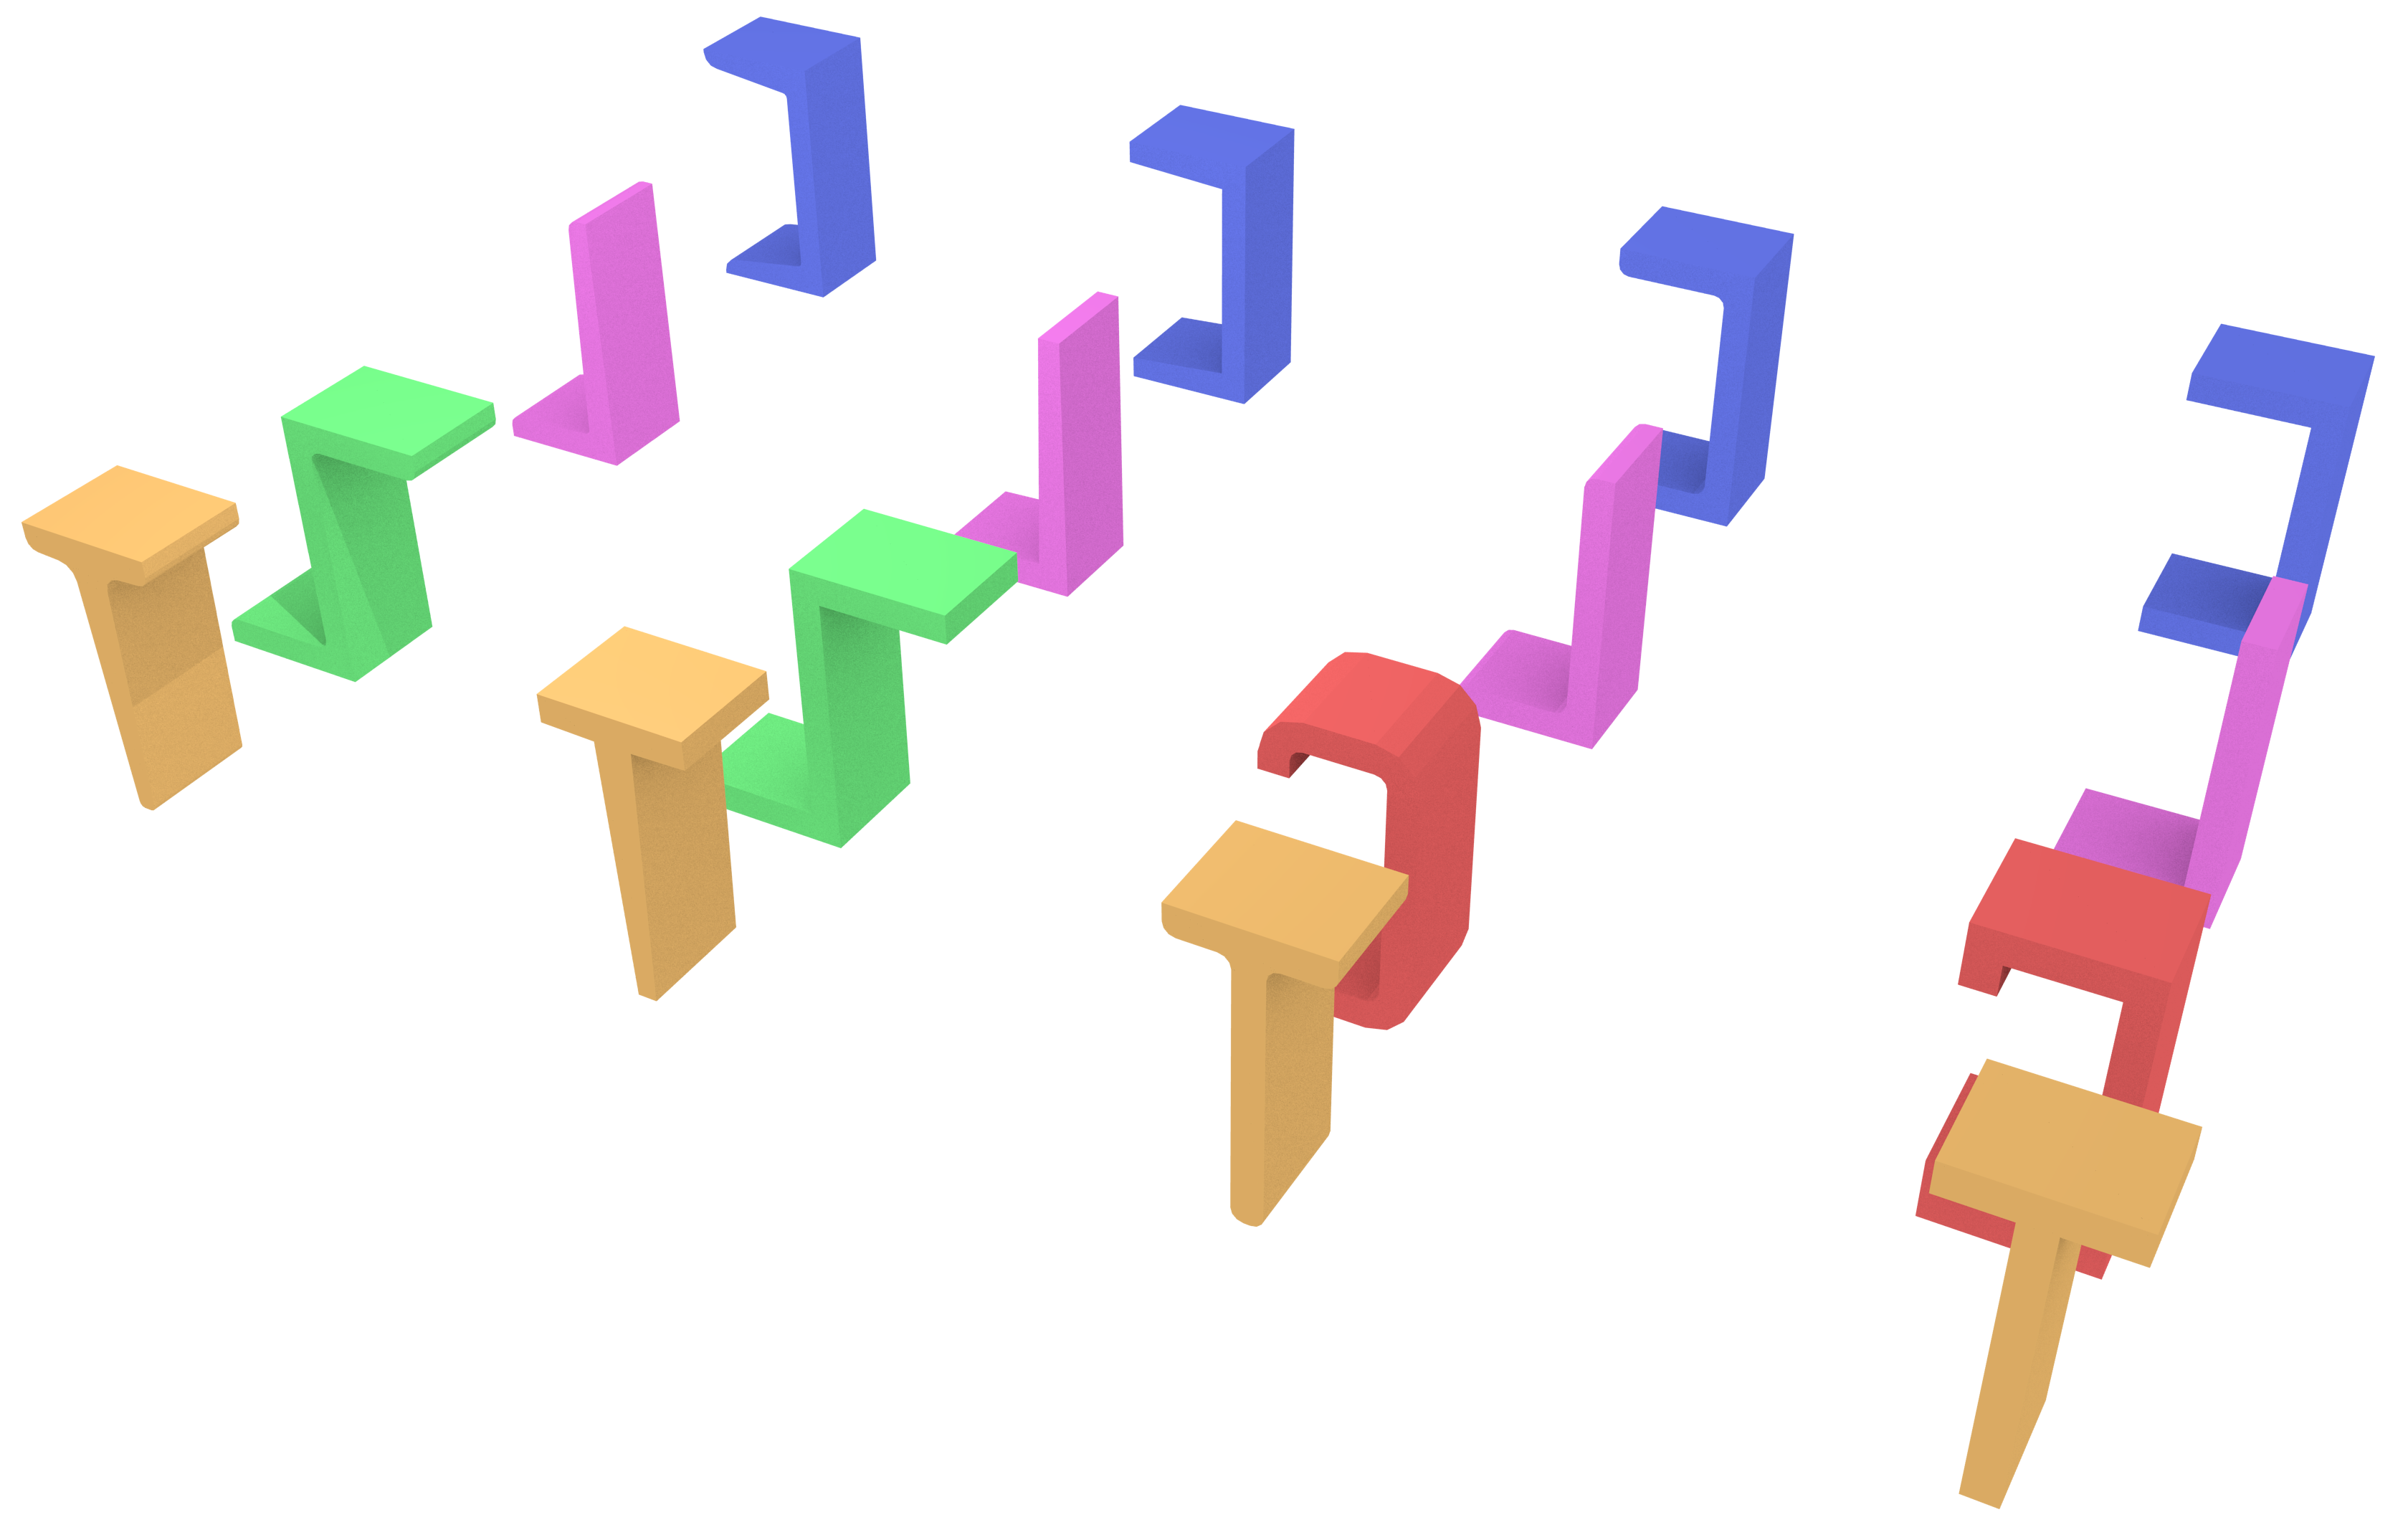
\includegraphics[width=\linewidth]{figs/letter_profiles}%
	\label{subfig:letter-profiles}
\end{subfigure}
\caption{The IFC standard supports parametric instantiated objects, such as these extrusions of (a) shape profiles and (b) letter profiles.}%
\label{fig:profiles}
\end{figure}

\begin{figure}
\begin{lstlisting}[frame=single]
#237=IFCEXTRUDEDAREASOLID(#236,#234,#230,6000.);
#238=IFCDIRECTION((1.,0.,0.));
#239=IFCDIRECTION((-1.,0.,1.));
#240=IFCCARTESIANPOINT((-2500.,0.,3000.));
#241=IFCAXIS2PLACEMENT3D(#240,#239,#238);
#242=IFCPLANE(#241);
#243=IFCHALFSPACESOLID(#242,.F.);
#244=IFCBOOLEANCLIPPINGRESULT(.DIFFERENCE.,#237,#243);
\end{lstlisting}
\caption{Removing part of a volume by subtracting a half-space from it using a Boolean operation.}%
\label{fig:csg}
\end{figure}

\begin{figure}
\centering
\begin{subfigure}[b]{0.45\linewidth}
	\includegraphics[width=\linewidth]{figs/ifc-1}%
	\label{subfig:ifc-1}
\end{subfigure}
\begin{subfigure}[b]{0.45\linewidth}
	\includegraphics[width=\linewidth]{figs/ifc-2}%
	\label{subfig:ifc-2}
\end{subfigure}
\caption{The IFC standard supports objects defined through sweeps, which are defined by (a) an \texttt{IfcPCurve} (black spiral) and a \texttt{SweptArea} (blue disk), in this case resulting in (b) a screw shape.}%
\label{fig:sweeps}
\end{figure}

\begin{figure}
\begin{lstlisting}[frame=single]
#120= IFCCARTESIANPOINT((-3.,13.,0.));
#122= IFCCARTESIANPOINT((12.,10.,0.));
#124= IFCCARTESIANPOINT((15.,13.,0.));
#126= IFCPOLYLOOP((#120,#122,#124));
\end{lstlisting}
\caption{Defining a simple polygon (\ie\ \texttt{IfcPolyLoop}) using B-rep.
Every point is defined as an \texttt{IfcCartesianPoint}, then the polygon is defined by a list of points.}%
\label{fig:brep}
\end{figure}

Related to how geometries are stored in IFC, two constructs (and related IFC classes) are particularly important: \texttt{IfcOpenings} and \texttt{IfcSpaces}.
Subtraction relationships are part of the IFC model, representing openings by means of the voiding mechanism:
\texttt{IfcOpening} defines the 3D objects that are subtracted from another geometry (\eg\ a hole for a window in an \texttt{IfcWall} or for a staircase in an \texttt{IfcSlab}).
The \texttt{IfcOpening} can be in turn filled by an element, like an \texttt{IfcWindow} or \texttt{IfcDoor}.
Meanwhile, \texttt{IfcSpaces} are used to explicitly model meaningful spaces (\eg\ rooms, apartments or storeys), and it is possible to associate attributes to them.

\subsection{Semantics}

The semantics in an IFC file are stored as a mix of entities, attributes and relationships.

An example of entities (classes) is given by all the subentities of \texttt{Ifc\-Buil\-ding\-E\-le\-ment}, including: \texttt{Ifc\-Beam}, \texttt{Ifc\-Buil\-ding\-E\-le\-ment\-Com\-po\-nent}, \texttt{Ifc\-Buil\-ding\-E\-le\-ment\-Pro\-xy}, \texttt{Ifc\-Chim\-ney}, \texttt{Ifc\-Co\-lumn}, \texttt{Ifc\-Co\-ve\-ring}, \texttt{Ifc\-Cur\-tain\-Wall}, \texttt{Ifc\-Door}, \texttt{Ifc\-Foo\-ting}, \texttt{Ifc\-Mem\-ber}, \texttt{Ifc\-Pile}, \texttt{Ifc\-Plate}, \texttt{Ifc\-Rai\-ling}, \texttt{Ifc\-Ramp}, \texttt{Ifc\-Ramp\-Flight}, \texttt{Ifc\-Roof}, \texttt{Ifc\-Sha\-ding\-De\-vice}, \texttt{Ifc\-Slab}, \texttt{Ifc\-Stair}, \texttt{Ifc\-Stair\-Flight}, \texttt{Ifc\-Wall}, and \texttt{Ifc\-Win\-dow}.
These can be used to represent many different functions that a building element can have, although there is also a commonly used generic one, \texttt{IfcBuildingElementProxy}, that does not provide this information.
% Its use should therefore be discouraged for elements that correspond to one of the entities listed above.
Similar subentities exist in other parts of the standard, such as for distribution elements (\eg\ for heating, cooling, ventilation and plumbing).

In order to represent objects which are not included in the IFC model, an \texttt{IfcProxy} element is foreseen, which is a subclass of \texttt{IfcProduct}.
For example, the entity \texttt{IfcBuildingElementProxy} described above is a subentity of \texttt{IfcProxy} for building elements.
Such generic entities are useful in order to support the addition of customised entities to models.
However, many times this is misused to represent objects which have suitable entities in the IFC model.
This is a problem, since a correct interpretation of such entities from the semantic point of view becomes more difficult, requiring either manual work or complex inferences based on their geometry.

Moreover, it is often possible to store the same kind of object by means of several entities.
For example, the layers within a compound wall object can be represented by means of an associated \texttt{IfcMaterialLayerSet}, but also as a more generic decomposition where every wall layer is modelled as a distinct \texttt{IfcBuildingElementPart}.

Regarding relationships between entities, IFC classes are generally structured in a deep hierarchies (is-a relationships), but some are organized in meronymic (part-of) trees, and there is support for spatial composition (fits-within) by means of \texttt{IfcSpatialStructureElements}\marginnote{\url{https://standards.buildingsmart.org/IFC/RELEASE/IFC4/ADD1/HTML/schema/ifcproductextension/lexical/ifcspatialstructureelement.htm}}.
This is used for the hierarchy of site, building, storey, space and zone.
Finally, elements are also related to one another directly, for example for wall connectivity and space boundaries.

Regarding attributes, various forms of semantic information can be associated to IFC elements, such as materials, properties (key-value pairs) and even scheduling.
The specific attributes that can be attached to each entity can be checked by looking at its documentation, taking into account that an entity can have all the attributes (recursively) inherited from its parents.

In addition, property sets can be used for attributes.
For instance, a building's use can be defined using the property set \texttt{Pset\_BuildingUse}, which includes things like its market category (\eg\ residential or commercial).
Another example is given in Figure~\ref{fig:pset}, where custom properties are defined in order to store specific semantics of a model.

\begin{figure}
	\begin{lstlisting}[frame=single]
	#991622=IFCPROPERTYSINGLEVALUE('End Extension Calculation',$,IFCLENGTHMEASURE(3000.),$);
	#991623=IFCPROPERTYSINGLEVALUE('Material',$,IFCLABEL('NL_01_hout_plaat'),$);
	#991624=IFCPROPERTYSINGLEVALUE('Length',$,IFCLENGTHMEASURE(2594.),$);
	#991625=IFCPROPERTYSINGLEVALUE('Start Release',$,IFCINTEGER(3),$);
	#991626=IFCPROPERTYSINGLEVALUE('End Release',$,IFCINTEGER(1),$);
	#991627=IFCPROPERTYSINGLEVALUE('Cut Length',$,IFCLENGTHMEASURE(2594.000000000001),$);
	#991628=IFCPROPERTYSINGLEVALUE('Structural Usage',$,IFCINTEGER(10),$);
	#991629=IFCPROPERTYSINGLEVALUE('Analyze As',$,IFCINTEGER(1),$);
	#991630=IFCPROPERTYSINGLEVALUE('Volume',$,IFCVOLUMEMEASURE(13602936.00000029),$);
\end{lstlisting}
	\caption{Defining properties to store the semantics in an IFC model.}%
	\label{fig:pset}
\end{figure}


% This semantic complexity is intended to represent faithfully the buildings as functional to the designed scope.
% However, the implementation and use of such theoretically precise models is difficult and can result in inaccuracies or the underuse of the most complex features, besides hindering interoperability by providing a very high degree of freedom to fill in the information in different ways and by choosing one of the many possible kinds of representations that can be used.

% \subsubsection{Model View Definitions}

% In order to define subsets of the IFC models to be implemented, the Information Delivery Manual (IDM) is added as part of the buildingSMART standard.
% It defines the workflow and the information exchange specifications and requirements for needed use cases.
% From each IDM, a set of Model View Definitions (MVD) can be defined for identifying the portion of the IFC model which is needed for the information exchange described in the IDM to be fulfilled.

% The documentation of an MVD allows the exchange to be repeated, providing consistency and predictability across a variety of projects and software platforms.
% MVDs are provided as part of the IFC releases and at present, the mostly implemented by software are the `Coordination view' for IFC version 2x3 and the `Design Transfer view' and `Reference view' for IFC version 4, designed with slightly different aims.

% The standard foresees the possibility of defining custom MVDs based on own specific requirements of the use case, although the implementation possibilities (by means of the mvdxml constructs) still present some weakness.


% \subsubsection{Disciplinary models and federated model}\label{sec:fedmodels}

% BIM models are usually split into several models, each of which describe the information related to a design discipline working on a project: architectural, structural, installations, etc.
% They are combined together in a federated model.

% For using the BIM, and in particular the IFC files representing each model, which are separately exported, it is important to know what to expect within each model: what elements are included and which ones are not.
% Note that these are potentially sharing the same space.
%
%The correct merger of multiple models into one is important for many use cases.
%For example, the computation of routes within the building should consider all the walls, whether they are load-bearing or not, and the calculation of volumes and heights have to count on all walls and slabs.
%Also with respect to integration with geoinformation, it is important to know which surrounding elements from the context where the building is designed are stored in the BIM\@.
%Another example is the computation of the maximum envelope of the building, such as for building permit regulation checks \citep{noardo2020investigating}, where all the elements that extend towards the outside of the building should be included (\eg\ chimneys and balconies).

% Unfortunately for interoperability, a unique subdivision of elements within such models is neither provided by standardization nor by shared practice.
% Instead, requirements and specifications are defined in each call for tenders according to the specific requirements of a particular use case.
% Although suboptimal, it is currently the most reasonable choice in order for users to obtain exactly the representation(s) they need.
% However, it means that: first, the elements can be stored in any of the models composing the federated one; and second, an element (such as a slab or a wall or an installation part) can be stored redundantly (and possibly inconsistently) within several discipline models.
%Arguably, in these circumstances, a validity checker should not detect the duplication of the same elements as a clash.
% Due to the way references between elements are stored within IFC models, in most cases, references can only be made between elements stored in the same file. This can cause issues when one depends on relationships (such as space boundaries) when the elements are contained in distinct aspect models.
%\citet{krijnen2020validation} provides options to later infer such relationships.
%
%The developers of tools to automatically process IFC models should consider this practice and possibly propose guidelines and prescriptions about the objects to be included in the representation for each case, or about how to document the modelling choices as machine-readable metadata.

\subsection{Georeferencing}

Properly georeferencing an IFC file makes it possible to link the (local) coordinates inside an IFC model with their corresponding real-world coordinates, and thus to place the model of a single building or construction within the virtual environment.
However, it is important to say that since georeferencing has historically not been necessary for designers, many IFC models are not georeferenced properly (or at all), which is a major issue in practice.

There are several options to store georeferencing information in IFC, as originally described by \citet{clemen2019level} and summarised in Table~\ref{tab:LoGeoRefs}.
These options range from basic address information to the definition of a more detailed position referred to a projected coordinate reference system (CRS).
In this last case, an offset can be stored between the project coordinate system and the global origin of a CRS (\(X\), \(Y\) and height).
The rotation of the \(XY\)-plane is also included.

\begin{table}
	\centering
	\small
	\begin{tabular}{m{1.6cm}m{2.2cm}m{5.5cm}}
		\toprule
		\textbf{LoGeoRef} & \textbf{Supported CRS} & \textbf{Storing entities} \\ \midrule
		LoGeoRef10 & No CRS, approximate location by means of the address. & \texttt{IfcPostalAddress} referenced by either \texttt{IfcSite} or \texttt{IfcBuilding}. \\ \addlinespace 
		LoGeoRef20& WGS84 EPSG:4326 & \texttt{RefLatitude, Ref\-Lon\-gi\-tude, Ref\-E\-le\-va\-tion} within \texttt{IfcSite} \\ \addlinespace
		LoGeoRef30 & Any Cartesian CRS, including projected coordinates (CRS not specified in the file) & \texttt{IfcCartesianPoint} referenced within \texttt{IfcSite} (defining the projected coordinates of the model reference point); \texttt{IfcDirection} attribute of \texttt{IfcSite}.% (stores rotations with respect to the project or global north).
		\tablefootnote{Ad-hoc solution used by several tools.} \\ \addlinespace 
		LoGeoRef40 & Any Cartesian CRS, including projected coordinates (CRS not specified in the file) & \texttt{WorldCoordinateSystem} storing the coordinates of the reference point in any Cartesian CRS (including the projected ones) and the orientation in \texttt{TrueNorth}. Both are stored within \texttt{IfcGeometricRepresentationContext}.\tablefootnote{Most official IFC2x3-way to store the reference system.} \\ \addlinespace 
		LoGeoRef50 & Specific projected CRS, specified by means of the EPSG code & IFC v.4 only%\tablefootnote{The IFC4 way of documenting the used CRS and other georeferencing parameters was proposed to be backported to property sets also for the version 2x3 of IFC\@. (\url{https://forums.buildingsmart.org/t/geolocation-standards-in-ifc2x3-and-ifc4/2329}). This could enable the achievement of \texttt{LoGeoRef50} even for IFC2x3 files.}.
		Coordinates of the reference point stored in \texttt{IfcMapConversion} using the attributes \texttt{Eastings},	\texttt{Northings} and \texttt{OrthogonalHeight} for global elevation. Rotation for the XY-plane stored using the attributes \texttt{XAxisAbscissa} and \texttt{XAxisOrdinate}. The coordinate reference system (CRS) used is specified by \texttt{IfcProjectedCRS} in the attribute \texttt{Name} by means of the proper EPSG code.  \\ \bottomrule
	\end{tabular}
	\caption{Synthesis of \texttt{LoGeoRefs} as defined by \citet{clemen2019level}.}%
	\label{tab:LoGeoRefs}
\end{table}


However, it is important to note that these levels of georeferencing do not necessarily indicate a scale measuring the quality of georeferencing, but they are mostly relevant to identify how the information is stored.
In fact, in some cases, the accuracy of different \texttt{LoGeoRefs} can be very similar (e.g.\ \texttt{LoGeoRef30} and \texttt{LoGeoRef40}), since the values are supposed to be the same, but stored differently within the IFC file.

%A further note is useful about the storage of the model reference system direction.
%In the \texttt{LoGeoRef40} the stored direction represents the \texttt{TrueNorth}\marginnote{\url{https://standards.buildingsmart.org/IFC/RELEASE/IFC2x2/FINAL/HTML/ifcrepresentationresource/lexical/ifcgeometricrepresentationcontext.html}} attribute, defined as \texttt{``Direction of the true north relative to the world coordinate system as established by the representation context''}.
%As also cited in the buildingSMART document about georeferencing\marginnote{\url{https://www.buildingsmart.org/wp-content/uploads/2020/02/User-Guide-for-Geo-referencing-in-IFC-v2.0.pdf}}, this could be different from the grid north, considering a Cartesian system and possibly stored as part of the \texttt{IfcObjectPlacement} within \texttt{IfcSite} (inherited from the class \texttt{IfcSpatialStructureElement} and, in turn, \texttt{IfcProduct}), according to \texttt{LoGeoRef30}.
% As defined in the IFC specifications\marginnote{\url{https://standards.buildingsmart.org/IFC/RELEASE/IFC2x/ADD1/HTML/ifcgeometricconstraintresource/lexical/ifcobjectplacement.html}} \emph{``The object placement can be given:
	% absolute (\ie\ by an axis2 placement, relative to the world coordinate system);
	% relative (\ie\ by an axis2 placement, relative to the object placement of another product);
	% by grid reference (\ie\ by the virtual intersection and reference direction given by two axes of a design grid).
	% In any case the object placement has to unambiguously define the object coordinate system as either two-dimensional axis placement (IfcAxis2Placement2D) or three-dimensional axis placement (IfcAxis2Placement3D).''}

% In the case of \texttt{IfcSite}, usually it is specified as \texttt{IfcLocalPlacement}\marginnote{\url{https://standards.buildingsmart.org/IFC/RELEASE/IFC2x/ADD1/HTML/ifcgeometricconstraintresource/lexical/ifclocalplacement.html}}, with attributes: \texttt{PlacementRelTo} (which, if omitted, indicates the World Coordinate System to be in theory defined within the geometric representation context) and \texttt{RelativePlacement}, filled by means of an \texttt{IfcAxis2Placement} class, specified as \texttt{IfcAxis2Placement3D}\marginnote{\url{https://standards.buildingsmart.org/IFC/RELEASE/IFC2x/ADD1/HTML/ifcgeometryresource/lexical/ifcaxis2placement3d.html}}.
% There, the attributes represented are usually: Location (inherited by \texttt{IfcPlacement} and stored as \texttt{IfcCartesianPoint}); Axis (representing the direction of the local $Z$ axis); \texttt{RefDirection}, storing the direction of the $X$ axis.
% It is relevant to note that in this case the direction of $X$ is stored, whilst in the \texttt{LoGeoRef40} case, under \texttt{IfcGeometricRepresentationContext} - \texttt{TrueNorth} attribute, the $Y$ direction of a possible Cartesian system is stored.
% Therefore, the values of two vectors composing the \texttt{IfcDirection} are inverted in the two cases.
% This must be considered when developing software applications reading the data in the two cases.

% In the specifications, it is established that, whether omitted, the reference should be the geometric coordinate system (used in \texttt{LoGeoRef40}).
% It is therefore necessary to be careful in the priority given to the information stored in the two systems: \texttt{LoGeoRef30} should be read first, if absent, then go to \texttt{LoGeoRef40}.








%In order to georeference an IFC file, it is possible to use the IFC entity \texttt{IfcSite}, which defines an area where construction works are undertaken, and optionally allows for storage of the real-world location of a project using the \emph{RefLatitude}, \emph{RefLongitude} and \emph{RefElevation} attributes.
%The latitude and longitude are defined as angles with degrees, minutes, seconds, and optionally millionths of seconds with respect to the world geodetic system WGS84 (EPSG:4326).
%Positive values represent locations north of the equator, west of the geodetic zero meridian (nominally the Greenwich prime meridian) in IFC2x3, or east of the zero meridian IFC4.
%Negative values represent locations south of the equator, east of the zero meridian in IFC2x3, or west of the zero meridian in IFC4.
%All the components of these angles (\ie\ degrees, minutes, seconds and millionth-seconds of arc) should have the same sign.
%According to the IFC standard, the geographic reference given might be the exact location of the origin of the local placement of the \texttt{IfcSite} or it might be an approximate position for informational purposes only.
%The elevation is defined according to the datum elevation relative to sea level.
%
%The IFC entity \texttt{IfcGeometricRepresentationContext} is used to define the coordinate space of an IFC model in 3D and optionally the 2D plan of such a model.
%This entity can be used to offset the project coordinate system from the global point of origin using the \emph{WorldCoordinateSystem} attribute, it defines the \emph{Precision} under which two given points are still assumed to be identical, and it defines the direction of the \emph{TrueNorth} relative to the underlying coordinate system.
%The latter attribute defaults to the positive direction of the y-axis of the \emph{WorldCoordinateSystem}.

\section{Exercises}

\begin{enumerate}

\item
Open a simple IFC file (\eg\ the IfcOpenHouse) in a text editor.
Can you understand the general structure of the file and how the STEP encoding works? 

\item
Find a line that defines an \texttt{IfcAxis2Placement3D}.
With the help of the documentation of that entity in the buildingSMART website, can you understand what it means?

\item
Much like 3D GIS standards like CityGML, IFC files represent a hierarchy.
However, the hierarchy in an IFC file looks much flatter with a simple entity in every line.
Is this really a flatter hierarchy?
What are some advantages and disadvantages of this (different) approach?

\end{enumerate}
